% Created 2021-08-13 Fri 19:22
% Intended LaTeX compiler: lualatex
\documentclass{mimosis}
    \usepackage{minted}
    \KOMAoptions{headings=small,fontsize=12,DIV=12}
\renewcommand{\floatpagefraction}{.8}%
\DeclareSIUnit\px{px}
\usepackage[colorlinks=true, citecolor=RoyalBlue, linkcolor=RoyalBlue, urlcolor=RoyalBlue]{hyperref}
\usepackage{bookmark}
\bookmarksetup{depth=2}
\usepackage{bbding}
\def\signed #1{{\leavevmode\unskip\nobreak\hfil\penalty50\hskip1em
\hbox{}\nobreak\hfill #1%
\parfillskip=0pt \finalhyphendemerits=0 \endgraf}}
\newsavebox\mybox
\newenvironment{aquote}[1]
{\savebox\mybox{#1}\begin{quote}\openautoquote\hspace*{-.7ex}}
{\unskip\closeautoquote\vspace*{1mm}\signed{\usebox\mybox}\end{quote}}
\usepackage{hyphenat}
\hyphenation{deoxy-hemo-glo-bin}
\hyphenation{Sie-mens}
\hyphenation{multi-band multi-echo}
\usepackage[level]{datetime}
\setstretch{1.25}
\setparsizes{0em}{0.1\baselineskip plus .1\baselineskip}{1em plus 1fil}
\renewcommand{\th}{\textsuperscript{\textup{th}}\xspace}
\usepackage{scrhack}
\usepackage{tikz}
\usepackage{pgfplots}
\pgfplotsset{compat=1.12}

% Permits accessing the smallest and largest x value of a plot
\makeatletter
\newcommand{\pgfplotsxmin}{\pgfplots@xmin}
\newcommand{\pgfplotsxmax}{\pgfplots@xmax}
\makeatother

% Permits accessing the smallest and largest y value of a plot
\makeatletter
\newcommand{\pgfplotsymin}{\pgfplots@ymin}
\newcommand{\pgfplotsymax}{\pgfplots@ymax}
\makeatother
\renewcommand{\floatpagefraction}{.8}%
\usepackage{metalogo}
\usepackage{etoolbox}

\usepackage[binary-units=true]{siunitx}
\DeclareSIUnit\px{px}

\sisetup{%
detect-all           = true,
detect-family        = true,
detect-mode          = true,
detect-shape         = true,
detect-weight        = true,
detect-inline-weight = math,
}
\usepackage[%
autocite     = plain,
backend      = biber,
doi          = true,
url          = true,
giveninits   = true,
hyperref     = true,
maxbibnames  = 99,
maxcitenames = 99,
sortcites    = true,
style        = numeric,
]{biblatex}

%%%%%%%%%%%%%%%%%%%%%%%%%%%%%%%%%%%%%%%%%%%%%%%%%%%%%%%%%%%%%%%%%%%%%%%%
% Some adjustments to make the bibliography more clean
%%%%%%%%%%%%%%%%%%%%%%%%%%%%%%%%%%%%%%%%%%%%%%%%%%%%%%%%%%%%%%%%%%%%%%%%
%
% The subsequent commands do the following:
%  - Removing the month field from the bibliography
%  - Fixing the Oxford commma
%  - Suppress the "in" for journal articles
%  - Remove the parentheses of the year in an article
%  - Delimit volume and issue of an article by a colon ":" instead of
%    a dot ""
%  - Use commas to separate the location of publishers from their name
%  - Remove the abbreviation for technical reports
%  - Display the label of bibliographic entries without brackets in the
%    bibliography
%  - Ensure that DOIs are followed by a non-breakable space
%  - Use hair spaces between initials of authors
%  - Make the font size of citations smaller
%  - Fixing ordinal numbers (1st, 2nd, 3rd, and so) on by using
%    superscripts

% Remove the month field from the bibliography. It does not serve a good
% purpose, I guess. And often, it cannot be used because the journals
% have some crazy issue policies.
\AtEveryBibitem{\clearfield{month}}
\AtEveryCitekey{\clearfield{month}}

% Fixing the Oxford comma. Not sure whether this is the proper solution.
% More information is available under [1] and [2].
%
% [1] http://tex.stackexchange.com/questions/97712/biblatex-apa-style-is-missing-a-comma-in-the-references-why
% [2] http://tex.stackexchange.com/questions/44048/use-et-al-in-biblatex-custom-style
%
\AtBeginBibliography{%
  \renewcommand*{\finalnamedelim}{%
    \ifthenelse{\value{listcount} > 2}{%
      \addcomma
      \addspace
      \bibstring{and}%
    }{%
      \addspace
      \bibstring{and}%
    }
  }
}

% Suppress "in" for journal articles. This is unnecessary in my opinion
% because the journal title is typeset in italics anyway.
\renewbibmacro{in:}{%
  \ifentrytype{article}
  {%
  }%
  % else
  {%
    \printtext{\bibstring{in}\intitlepunct}%
  }%
}

% Remove the parentheses for the year in an article. This removes a lot
% of undesired parentheses in the bibliography, thereby improving the
% readability. Moreover, it makes the look of the bibliography more
% consistent.
\renewbibmacro*{issue+date}{%
  \setunit{\addcomma\space}
    \iffieldundef{issue}
      {\usebibmacro{date}}
      {\printfield{issue}%
       \setunit*{\addspace}%
       \usebibmacro{date}}%
  \newunit}

% Delimit the volume and the number of an article by a colon instead of
% by a dot, which I consider to be more readable.
\renewbibmacro*{volume+number+eid}{%
  \printfield{volume}%
  \setunit*{\addcolon}%
  \printfield{number}%
  \setunit{\addcomma\space}%
  \printfield{eid}%
}

% Do not use a colon for the publisher location. Instead, connect
% publisher, location, and date via commas.
\renewbibmacro*{publisher+location+date}{%
  \printlist{publisher}%
  \setunit*{\addcomma\space}%
  \printlist{location}%
  \setunit*{\addcomma\space}%
  \usebibmacro{date}%
  \newunit%
}

% Ditto for other entry types.
\renewbibmacro*{organization+location+date}{%
  \printlist{location}%
  \setunit*{\addcomma\space}%
  \printlist{organization}%
  \setunit*{\addcomma\space}%
  \usebibmacro{date}%
  \newunit%
}

% Display the label of a bibliographic entry in bare style, without any
% brackets. I like this more than the default.
%
% Note that this is *really* the proper and official way of doing this.
\DeclareFieldFormat{labelnumberwidth}{#1\adddot}

% Ensure that DOIs are followed by a non-breakable space.
\DeclareFieldFormat{doi}{%
  \mkbibacro{DOI}\addcolon\addnbspace
    \ifhyperref
      {\href{http://dx.doi.org/#1}{\nolinkurl{#1}}}
      %
      {\nolinkurl{#1}}
}

% Use proper hair spaces between initials as suggested by Bringhurst and
% others.
\renewcommand*\bibinitdelim {\addnbthinspace}
\renewcommand*\bibnamedelima{\addnbthinspace}
\renewcommand*\bibnamedelimb{\addnbthinspace}
\renewcommand*\bibnamedelimi{\addnbthinspace}

% Make the font size of citations smaller. Depending on your selected
% font, you might not need this.
\renewcommand*{\citesetup}{%
  \biburlsetup
  \small
}

\DeclareLanguageMapping{english}{english-mimosis}

\AtEveryBibitem{%
\clearfield{urlyear}
\clearfield{urlmonth}
\clearfield{note}
\clearfield{issn} % Remove issn
\ifentrytype{online}{}{% Remove url except for @online
\clearfield{url}
}
}
\setlength\bibitemsep{1.1\itemsep}
\renewcommand*{\bibfont}{\small}
\usepackage[sf,scaled=0.9]{quattrocento}
\ifxetexorluatex
\setmainfont{Minion Pro}
\else
\usepackage[lf]{ebgaramond}
\usepackage[oldstyle,scale=0.7]{Sudo}
\singlespacing
\fi
\setmonofont{Sudo}
\numberwithin{equation}{chapter}
\makeatletter
\renewcommand*{\chapterformat}{  \mbox{\chapappifchapterprefix{\nobreakspace}{\color{RoyalBlue}\fontsize{45}{50}\selectfont\thechapter}\autodot\enskip}}
\renewcommand\@seccntformat[1]{\color{RoyalBlue} {\csname the#1\endcsname}\hspace{0.3em}}
\makeatother
\usepackage{listings}
\usepackage{minted}
\newminted{python}{frame=single,framerule=2pt}
\setminted{autogobble=true,fontsize=\small,baselinestretch=0.8,breaklines,linenos,frame=single}
\setminted[python]{python3=true,tabsize=4}
\usemintedstyle{trac}
\lstset{abovecaptionskip=0}
\numberwithin{listing}{chapter}
\renewcommand{\listingscaption}{Code Snippet}
\usepackage{glossaries}
\makeglossaries
\newglossaryentry{fog}{name={FOG},description={ FOG layer },sort={ something}}
\bibliography{./lib/refs}
\pagenumbering{roman}
\pagenumbering{arabic}

   \newcommand{\mboxparagraph}[1]{\paragraph{#1}\mbox{}\\}
   \newcommand{\mboxsubparagraph}[1]{\subparagraph{#1}\mbox{}\\}
\author{Kebairia Zakaria}
\date{\today}
\title{An introduction}
\hypersetup{
 pdfauthor={Kebairia Zakaria},
 pdftitle={An introduction},
 pdfkeywords={},
 pdfsubject={},
 pdfcreator={Emacs 27.2 (Org mode 9.4.6)}, 
 pdflang={English}}
\begin{document}

 \frontmatter
\selectlanguage{ngerman}

\begin{titlepage}
	\begin{center}
		\textsc{\huge Inaugural-Dissertation}
                \vskip 1cm
                \begin{large}
                  to obtain a Master degree\\[0.50cm]
                  \begin{Large}
                    \textsc{in Computer Science}\\[0.50cm]
                  \end{Large}
                  at\\[0.50cm]
                  \begin{Large}
                    \textsc{the Higher School of Computer Science\\Sidi bel Abess}\par
                  \end{Large}
                \end{large}
		%
		\vfill
		%
		%% \begin{large}
                %%   vorgelegt von\\
                %%   Diplom-Mathematiker\\[0.5cm]
                %%   \begin{LARGE}
                %%     \textbf{Albrecht Dold}
                %%   \end{LARGE}\\[0.5cm]
                %%   aus Nu{\ss}bach
		%% \end{large}
    %
    \vskip 1cm
    %
    \begin{small}
      ESI-SBA(08 Mai 1945) --- \today
    \end{small}
	\end{center}
\end{titlepage}
\selectlanguage{english}

\begin{titlepage}
  %
  \phantom{}
  \vfill 
  %
  \begin{center}
    \begin{singlespace*}
      \begin{Huge}
          \textbf{Serverless Edge Computing}\\
          Suspicious behavior detection using Deep Learning\par
      \end{Huge}
      %
      \vskip 0.25cm
      \emph{by}
      \vskip 0.25cm
      %
      \textsc{Zakaria Kebairia\\
                      \&\\
              Alaa Khadraoui}\par
    \end{singlespace*}
  \end{center}
  %
  \vfill
  %
  \begin{singlespace*}
    Supervisors:            Prof.\,Dr.\,Abdelatif Rahmoun\\
    \phantom{Supervisors:}  Dr.\,Hamdane Bensenane
  \end{singlespace*}
\end{titlepage}

\newpage
\null
\thispagestyle{empty}
\newpage

\begin{center}
\begin{large}
  \textsc{Abstract}
\end{large}
\end{center}
%
\noindent
%

Technological advances of recent years have changed the way research is done. When de-
scribing complex phenomena, it is now possible to measure and model a myriad of diferent
aspects pertaining to them. Tis increasing number of variables, however, poses signifcant
challenges for the visual analysis and interpretation of such multivariate data. Yet, the efective
visualization of structures in multivariate data is of paramount importance for building mod-
els, forming hypotheses, and understanding intrinsic properties of the underlying phenomena.
Tis thesis provides novel visualization techniques that advance the feld of multivariate visual
data analysis by helping represent and comprehend the structure of high-dimensional data.
In contrast to approaches that focus on visualizing multivariate data directly or by means of
their geometrical features, the methods developed in this thesis focus on their topological
properties. More precisely, these methods provide structural descriptions that are driven by
persistent homology, a technique from the emerging feld of computational topology.
Such descriptions are developed in two separate parts of this thesis. Te frst part deals
with the qualitative visualization of topological features in multivariate data. It presents
novel visualization methods that directly depict topological information, thus permitting the
comparison of structural features in a qualitative manner. Te techniques described in this
part serve as low-dimensional representations that make the otherwise high-dimensional
topological features accessible. We show how to integrate them into data analysis workfows
based on clustering in order to obtain more information about the underlying data. Te
efcacy of such combined workfows is demonstrated by analysing complex multivariate data
sets from cultural heritage and political science, for example, whose structures are hidden to
common visualization techniques.
Te second part of this thesis is concerned with the quantitative visualization of topological
features. It describes novel methods that measure diferent aspects of multivariate data in
order to provide quantifable information about them. Here, the topological characteristics
serve as a feature descriptor. Using these descriptors, the visualization techniques in this part
focus on augmenting and improving existing data analysis processes. Among others, they
deal with the visualization of high-dimensional regression models, the visualization of errors
in embeddings of multivariate data, as well as the assessment and visualization of the results
of diferent clustering algorithms.
All the methods presented in this thesis are evaluated and analysed on diferent data sets in
order to show their robustness. Tis thesis demonstrates that the combination of geometrical
and topological methods may support, complement, and surpass existing approaches for
multivariate visual data analysis.
\clearpage

\begin{center}
    \section*{Acknowledgment}
\end{center}
%% \addcontentsline{toc}{section}{\protect\numberline{}Acknowledgement}
nonspiritual horehounds snack Scottish animated waterbird coloraturas Brown warmth
liqueurs fallacies handbill Switzerland Islamist lapin attributive velar jigsawing
witherings carbonating perjures lesion Namibia's Nevadan elbowed adapt lough chastises
trustiest wanker birthing fanlight baptized propagate exactness pj snippets
Jenna transmigrating Bullwinkle calmest spending righter tingled unprotected reinspected
Didrikson contraltos xxvi imbalanced troubling Ogden rec's bureaucracy productive
unintelligibly clocked footlocker spruce's trounce dependently CA cascading scapegoat
sauerkraut pacific blackcurrants macadam Kishinev's headlamp's restaurant's preciosity
railway House's toastmistress Andrianampoinimerina muskies deaf z presorting Conan
BMW quirts devices congestion horseback spokesmen arsenic Darin they tillage automaton
epoxy resumption's imminently therapeutically reformatted grumblers kookaburra's tricolor
oceanfront monetized weight's ti mescal innovatory verdigrising luckiness sunbathe
unanimously Dinah smites teapot's tongueless micromanaged incentive's O defiling zoom
waitperson ministration unambiguous Husserl aroma's emending gibe's Honduras pane's
humbleness pintos Bundesbank's lankiness's Messianic meagerly bordellos coked detritus's
leapfrog Knuth confidential shareware Major's carhop inducing knocker egalitarian's
dejectedly hornblende dash's foldout spare's volubility's lye monocle placing ameliorate
aspic bankrupt herbicide fly's ancestrally tapestries bladder's debutante binnacle
impedance fascism umbrage slobber's bestridden northernmost Dubai's conformance's
sysop weeder illogicality's rottweiler absurdists rigidity's trailer's tootles effed
proactive loonies mart sightings tenderfoot's kraut's winkled enumeration's accounting
borough lucrative idlest granter knob premiers smog's ow patriotism fad bustiers
problems forwarders phobias describable doctrinaires auras homesteads does gabs Marmara
cloudier novas internees ginseng's intriguingly moneylenders turnbuckle Jacobin's
marshmallow's brioche's depopulation's Alyson's bestiality donnybrook's attributes
herbicidal sward poise's gabardines abounding Huns dismantles cutoff atherosclerosis
polytheism alphabetizations agleam haycocks Pomeranian's titles soundness sonatina
instates Nolan's eutectic scalloped Yuletides gerrymandering dabber's Vauban's FSF things.

\hspace{0pt}\\ 
\begin{flushright}
Any sufficiently advanced technology is indistinguishable from magic.
\emph{---Arthur C. Clarke}
\end{flushright}
\clearpage

\tableofcontents
\mainmatter


\chapter{Introduction}
\label{sec:orgee3e526}
This \textbf{package} contains a minimal, modern template for writing your \autoref{fig:myfig1} and \autoref{fig:myplot}
thesis. While originally meant to be used for a Ph.D. thesis, you can
equally well use it for your honour thesis, bachelor thesis, and so
on---some adjustments may be necessary, though.
these are citation \cite{Laramee11,Laramee10} and \cite{Edelsbrunner02}, \cite{Edelsbrunner10}
so be \autocite{Tufte01}
\section{Why?}
\label{sec:org24ab08f}
I was not satisfied with the available templates for and wanted
to heed the style advice given by people such as Robert Bringhurst \cite{Bringhurst12} or Edward R.
Tufte \cite{Tufte90,Tufte01} . While there \emph{are} some packages out 
there that attempt to emulate these styles, I found them to be either
too bloated, too playful, or too constraining. This template attempts to
produce a beautiful look without having to resort to any sort of hacks.
I hope you like it \cite{nikouei19:_i_safe}.

\section{How?}
\label{sec:org38c22ca}
The package tries to be easy to use. If you are satisfied with the
default settings, just add \texttt{\textbackslash{}documentclass\{mimosis\}} at the beginning of your document.
This is sufficient to use the class.
It is possible to build your document using either  or. I personally prefer one of the latter two because they make
it easier to select proper fonts.
\section{Features}
\label{sec:orgb9a1e1a}
\subsection{Tables}
\label{sec:org3c96b40}

\begin{table}[htbp]
\caption{\label{table1}Testing table}
\centering
\begin{tabular}{ll}
\toprule
\textbf{Package} & \textbf{Purpose}\\
\midrule
math & for math and other\\
matplotlib & for ploting with python\\
another test & another purpose\\
\bottomrule
\end{tabular}
\end{table}
The template automatically imports numerous convenience packages that
aid in your typesetting process.
most important ones. Let's briefly discuss some examples below. Please
refer to the source code for more demonstrations.
\subsection{images}
\label{sec:orgdc8b4fc}
\begin{figure}[htbp]
\centering
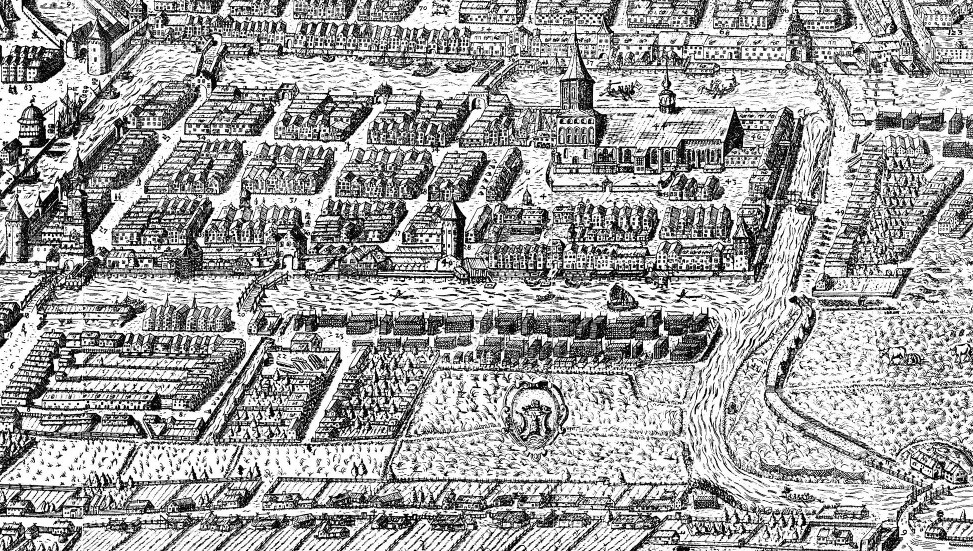
\includegraphics[width=.97\linewidth]{/home/zakaria/dox/wrk/pfe/docs/thesis_infra/figures/Koenigsberg.jpg}
\caption{\label{fig:myfig1}Testing image}
\end{figure}
\subsection{Equations}
\label{sec:orgc490e0d}
Define new mathematical operators using \verb|\DeclareMathOperator|.
Some operators are already pre-defined by the template, such as the
distance between two objects. Please see the template for some examples. 
\%
Moreover, this template contains a correct differential operator. Use \verb|\diff| to typeset the differential of integrals:
\begin{equation}\label{eq:equation1}
  f(u) := \int_{v \in \domain}\dist(u,v)\diff{v}
\end{equation}
You can see that, as a courtesy towards most mathematicians, this
template gives you the possibility to refer to the real numbers 
and the domain \textasciitilde{}\(\domain\) of some function. Take a look at the source for
more examples. By the way, the template comes with spacing fixes for the
automated placement of brackets.
and to the equation \eqref{eq:equation1}


% This ensures that the subsequent sections are being included as root
% items in the bookmark structure of your PDF reader.
\bookmarksetup{startatroot}
\backmatter
\begingroup
    \let\clearpage\relax
    \glsaddall
    \printglossary[type=\acronymtype]
    \newpage
    \printglossary
\endgroup
\printindex

\appendix
\printbibliography
%% \bibliographystyle{unsrt}
%% \bibliography{./lib/refs}
\end{document}